\documentclass[11pt]{article}
\usepackage[utf8]{inputenc}
\usepackage[spanish,es-nodecimaldot]{babel}
\usepackage[a4paper,margin=2.4cm]{geometry}
\usepackage{amsmath,booktabs,graphicx,siunitx,url}
\setlength{\textfloatsep}{6pt}
\setlength{\floatsep}{6pt}
\setlength{\intextsep}{6pt}
\setlength{\abovedisplayskip}{5pt}
\setlength{\belowdisplayskip}{5pt}
\title{Test 5: malla, contorno y evidencia}
\author{Emilio Catalán Contreras}
\date{}

\begin{document}
\maketitle

\section{Problema y objetivo}

Se estudió una barra axial lineal elástica con el extremo izquierdo restringido, una carga puntual en el extremo derecho y una carga axial uniforme. El objetivo fue determinar si el acuerdo de los desplazamientos en los nodos es suficiente para aceptar el campo aproximado y analizar qué ocurre al refinar la malla de 2 a 4 y 8 elementos. Además, se estudió el efecto de imponer una restricción adicional $u(L)=0$, distinguiendo el refinamiento de malla de un cambio en las condiciones de borde.

\section{Datos, supuestos y método}

Se utilizaron $L=2000$ mm, $E=200000$ N/mm$^2$, $A=1000$ mm$^2$, $P=20000$ N y $q=10$ N/mm. Se consideró un modelo axial lineal elástico, con $E$ y $A$ constantes. La solución mediante elementos finitos fue obtenida con el solver NumPy suministrado, utilizando la resolución del sistema lineal con \texttt{numpy.linalg.solve} \cite{numpy}.

La referencia independiente se obtuvo desde

\[
-(EAu')'=q,
\]

con $u(0)=0$ y $EAu'(L)=P$. Para estas condiciones,

\[
u_{\mathrm{ref}}(x)=
\frac{(P+qL)x-\frac{q x^2}{2}}{EA}.
\]

El error se evaluó en los puntos medios de cada elemento, interpolando linealmente el desplazamiento del modelo numérico y comparándolo con $u_{\mathrm{ref}}$. Este procedimiento permite evaluar el campo entre nodos y no solamente el acuerdo nodal, siguiendo el enfoque de verificación de modelos computacionales \cite{rod}.

\section{Resultados y verificación}

La Tabla 1 resume los resultados obtenidos.

\begin{table}[h]
\centering
\small
\begin{tabular}{cccc}
\toprule
Elementos & $u(L)$ [mm] & $R_{\mathrm{izq}}$ [N] & Error máx. [mm] \\
\midrule
2 & 0.300 & -40000 & 0.006250 \\
4 & 0.300 & -40000 & 0.0015625 \\
8 & 0.300 & -40000 & 0.000390625 \\
\bottomrule
\end{tabular}
\caption{Resultados para las tres mallas del problema base.}
\end{table}

El desplazamiento $u(L)$ se mantuvo prácticamente en 0.300 mm para las tres mallas. Sin embargo, el error máximo entre nodos disminuyó al refinar la discretización. Al duplicar el número de elementos, el error disminuyó aproximadamente a la cuarta parte.

La carga total aplicada es

\[
P+qL=20000+10(2000)=40000\ \mathrm{N},
\]

por lo que la reacción $R_{\mathrm{izq}}\approx-40000$ N permite cerrar el equilibrio global. Las pruebas suministradas también fueron ejecutadas mediante \texttt{pytest}, obteniéndose 2 pruebas aprobadas antes de ejecutar el estudio completo.

\begin{figure}[h]
\centering
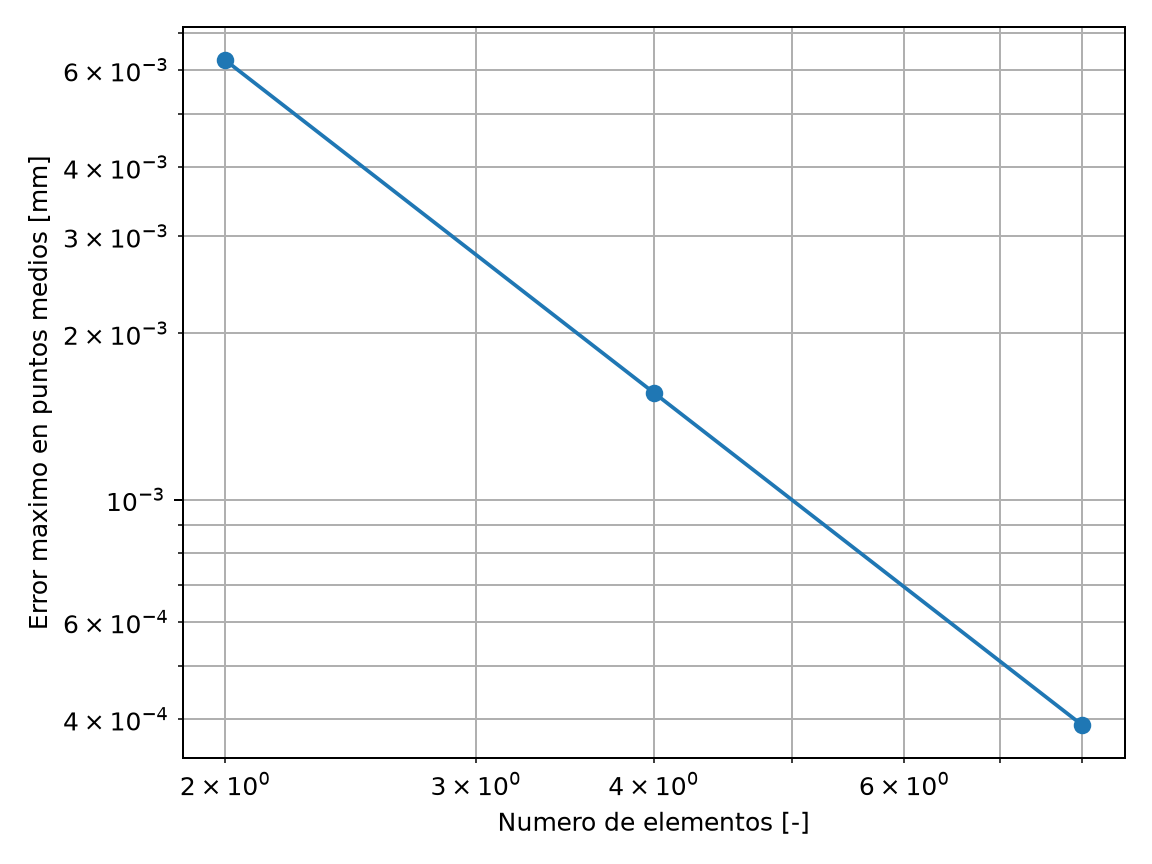
\includegraphics[width=0.47\textwidth]{../salidas/convergencia.png}
\caption{Error máximo en puntos medios frente al número de elementos.}
\end{figure}

\section{Interpretación y conclusiones}

La predicción inicial indicaba que el error disminuiría al aumentar la cantidad de elementos. Los resultados confirmaron esta tendencia. Aunque $u(L)$ coincide para las tres discretizaciones, el campo aproximado entre nodos no presenta el mismo nivel de exactitud, por lo que el acuerdo nodal por sí solo no es suficiente para aceptar completamente la solución.

En el caso de contorno alterado se agregó $u(L)=0$. Se obtuvo $R_{\mathrm{izq}}=-10000$ N y $R_{\mathrm{der}}=-30000$ N, manteniéndose el equilibrio global. Sin embargo, este resultado no corresponde a una mejora de la malla: la nueva restricción modifica el problema físico. Por lo tanto, un modelo puede satisfacer el equilibrio numérico y aun representar condiciones de borde distintas a las originales.

Como limitación, el análisis corresponde únicamente al modelo axial lineal suministrado y a las tres discretizaciones solicitadas; no permite generalizar el comportamiento a otros tipos de elementos o problemas estructurales.

\section*{Declaración de uso de IA}

Se utilizó ChatGPT (OpenAI) como apoyo para interpretar la consigna y el material de clases, revisar las funciones de referencia analítica y error en puntos medios, orientar la ejecución del proyecto y apoyar la redacción del informe. Las sugerencias incorporadas fueron contrastadas con las ecuaciones y condiciones de borde entregadas y verificadas mediante \texttt{pytest}, la ejecución de \texttt{src/ejecutar.py}, el archivo \texttt{resultados.csv}, el equilibrio global y el gráfico de convergencia.

\bibliographystyle{plain}
\bibliography{referencias}

\end{document}